%% Lab Report for EEET2493_labreport_template.tex
%% V1.0
%% 2019/01/16
%% This is the template for a Lab report following an IEEE paper. Modified by Francisco Tovar after Michael Sheel original document.


%% This is a skeleton file demonstrating the use of IEEEtran.cls
%% (requires IEEEtran.cls version 1.8b or later) with an IEEE
%% journal paper.
%%
%% Support sites:
%% http://www.michaelshell.org/tex/ieeetran/
%% http://www.ctan.org/pkg/ieeetran
%% and
%% http://www.ieee.org/

%%*************************************************************************
%% Legal Notice:
%% This code is offered as-is without any warranty either expressed or
%% implied; without even the implied warranty of MERCHANTABILITY or
%% FITNESS FOR A PARTICULAR PURPOSE! 
%% User assumes all risk.
%% In no event shall the IEEE or any contributor to this code be liable for
%% any damages or losses, including, but not limited to, incidental,
%% consequential, or any other damages, resulting from the use or misuse
%% of any information contained here.
%%
%% All comments are the opinions of their respective authors and are not
%% necessarily endorsed by the IEEE.
%%
%% This work is distributed under the LaTeX Project Public License (LPPL)
%% ( http://www.latex-project.org/ ) version 1.3, and may be freely used,
%% distributed and modified. A copy of the LPPL, version 1.3, is included
%% in the base LaTeX documentation of all distributions of LaTeX released
%% 2003/12/01 or later.
%% Retain all contribution notices and credits.
%% ** Modified files should be clearly indicated as such, including  **
%% ** renaming them and changing author support contact information. **
%%*************************************************************************

\documentclass[journal]{IEEEtran}

% *** CITATION PACKAGES ***
\usepackage[style=ieee]{biblatex} 
\bibliography{example_bib.bib}    %your file created using JabRef

% *** MATH PACKAGES ***
\usepackage{amsmath}
\usepackage{comment}

\usepackage{tabularx} % en el preámbulo
\usepackage{caption}
\captionsetup{font=small, labelfont=bf, textfont=normalfont}

% *** PDF, URL AND HYPERLINK PACKAGES ***
\usepackage{url}
% correct bad hyphenation here
\hyphenation{op-tical net-works semi-conduc-tor}
\usepackage{graphicx}  %needed to include png, eps figures
\usepackage{float}  % used to fix location of images i.e.\begin{figure}[H]

\begin{document}


% paper title
\title{Reguladores de Voltaje con Diodos Zener\\ \small{Práctica No. 3}}

% author names and affiliations
\author{
    \IEEEauthorblockN{Flores Cornejo Gustavo Mauricio, Muñoz Reyes Arturo Yabed, Morales Vásquez Miguel Ehecatl}\\
    \IEEEauthorblockA{\textit{Unidad Profesional Interdisciplinaria en Ingeniería y Tecnologías Avanzadas, IPN}}
}
        
% The report headers
\markboth{1MV12 Fundamentos de Electrónica. Práctica 3, Marzo 2026}%do not delete next lines
{Shell \MakeLowercase{\textit{et al.}}: Bare Demo of IEEEtran.cls for IEEE Journals}

% make the title area
\maketitle

% As a general rule, do not put math, special symbols or citations
% in the abstract or keywords.
\begin{abstract}
 
\end{abstract}

\section{Introducción}
% Here we have the typical use of a "W" for an initial drop letter
% and "RITE" in caps to complete the first word.
% You must have at least 2 lines in the paragraph with the drop letter
% (should never be an issue)

\IEEEPARstart{E}l 


\section{Objetivos}


\section{Marco teórico}


\section{Materiales}

\begin{comment}
\begin{figure}[H]%[!ht]
\begin {center}

\includegraphics[width=0.45\textwidth]{IMAGENES/CB_DIODO4001.jpeg}
\caption{Circuito con diodo 1N4001.}
\label{fig:circuito_base1}
\end {center}
\end{figure}
\end{comment}

Para el circuito mostrado en la "Figura~\ref{fig:circuito_base1}”, emplearemos:
\begin{itemize}
    \item 1 Diodo 1N4001
    \item 1 Diodo 1N4148
    \item 1 Resistencia de 220 $\Omega$
    \item Protoboard
    \item Cable para protoboard
\end{itemize}

\section{Análisis y Resultados del circuito}
\subsection{Características Básicas.}
En esta primera sección se mostrarán los resultados obtenidos de realizar las mediciones básicas que caracterizan a cada uno de los diodos, como los es Voltaje de Umbral, medido con la función de 
prueba de diododos del multímetro para una polarización directa y una invesa para ambos casos. Además de medir la impedancia presente en el diodo para ambas fases mencionadas anteriormente.

\begin{table}[H]
\centering
\begin{tabularx}{\columnwidth}{|c|X|X|X|}
\hline
\textbf{Diodo} & \textbf{Voltaje de Umbral (V)} & \textbf{Resistencia ($\Omega$)}\\ \hline
1N4001 & 0.544 & 0\\ \hline
1N4148 & 0.540 & 0\\ \hline
\end{tabularx}
\caption{Mediciones Básicas en Polaridad Directa.}
\label{PolaridadDirecta}
\end{table}

\begin{table}[H]
\centering
\begin{tabularx}{\columnwidth}{|c|X|X|X|}
\hline
\textbf{Diodo} & \textbf{Voltaje de Umbral (V)} & \textbf{Resistencia ($\Omega$)}\\ \hline
1N4001 & 0 & 1.80M\\ \hline
1N4148 & 0 & 1.74M\\ \hline
\end{tabularx}
\caption{Mediciones Básicas en Polaridad Inversa.}
\label{PolaridadInversa}
\end{table}
Esta parte es importante, pues con estas mediciones nos podemos dar cuenta si alguno de nuestro componentes está dañado, pues si registramos lecturas de Voltaje de Umbral 
fuera del rango 0.5V - 0.7V o si registramos una resistencia pequeña en la polarización inversa como lo indica la tabla del fabricante véase Tabla \ref{tablaComparacionDiodos}. 

\subsection{Polarización Directa}
Para esta primera parte se realizaron las mediciones de voltaje, corriente y resistencia estática de los diodos dada una polarización directa.
Partiendo de los valores de $V_D$ y $I_D$ es fácil calcular la resistencia estática del diodo, partiendo de la ley de ohm, obtenemos:
\begin{equation}
R_{\text{estática}} = \frac{V_D}{I_D}
\end{equation}

\begin{table}[H]
\centering
\begin{tabularx}{\columnwidth}{|c|X|X|X|X|}
\hline
\textbf{V1 (V)} & \textbf{$I_D$ (mA)} & \textbf{$V_D$ (V)} & \textbf{$V_\text{R1}$ (V)} & \textbf{$R_\text{Estatica}$ (Ohms)}\\ \hline
0.0 & 0.000 & 0.000  & 0.000 &  INFINITA\\ \hline
0.3 & 0.000 & 0.286  & 0.000 &  INFINITA\\ \hline
0.5 & 0.092 & 0.477  & 0.021 &  5184.8\\ \hline
0.7 & 0.342 & 0.536  & 0.074 &  1567.3\\ \hline
1.0 & 1.191 & 0.596  & 0.257 &  500.42\\ \hline
1.5 & 3.730 & 0.651  & 0.805 &  174.53\\ \hline
2.0 & 5.780 & 0.678  & 1.238 &  117.3\\ \hline
3.0 & 10.02 & 0.696  & 2.160 &  69.461\\ \hline
5.0 & 18.55 & 0.720  & 3.990 &  38.814\\ \hline
7.0 & 27.50 & 0.740  & 5.880 &  26.909\\ \hline
10.0& 40.90 & 0.750  & 8.690 &  19.337\\ \hline
\end{tabularx}
\caption{Tabla de mediciones del diodo 1N4001.}
\label{tablaDiodo4001}
\end{table}

\begin{table}[H]
\centering
\begin{tabularx}{\columnwidth}{|c|X|X|X|X|}
\hline
\textbf{V1 (V)} & \textbf{$I_D$ (mA)} & \textbf{$V_D$ (V)} & \textbf{$V_\text{R1}$ (V)} & \textbf{$R_\text{Estatica}$ (Ohms)}\\ \hline
0.0 & 0.000 & 0.000  & 0.000 &  INFINITA\\ \hline
0.3 & 0.000 & 0.300  & 0.000 &  INFINITA\\ \hline
0.5 & 0.080 & 0.479  & 0.020 &  5184.8\\ \hline
0.7 & 0.560 & 0.570  & 0.127 &  1567.3\\ \hline
1.0 & 1.650 & 0.623  & 0.375 &  500.42\\ \hline
1.5 & 3.650 & 0.662  & 0.825 &  174.53\\ \hline
2.0 & 5.780 & 0.686  & 1.300 &  117.3\\ \hline
3.0 & 9.990 & 0.718  & 2.250 &  69.461\\ \hline
5.0 & 18.63 & 0.750  & 4.180 &  38.814\\ \hline
7.0 & 27.40 & 0.780  & 6.130 &  26.909\\ \hline
10.0& 40.70 & 0.810  & 9.060 &  18.337\\ \hline
\end{tabularx}
\caption{Tabla de mediciones del diodo 1N4148.}
\label{tablaDiodo4148}
\end{table}

Los resultados mostrados son comprobables visualizando el circuito equivalente, pues, como sabemos el diodo se comporta como circuito abierto
hasta alcanzar su voltaje de umbral (aproximadamente 0.7V para diodos de silicio), después de esto, el diodo se comporta como un corto circuito, lo que se refleja en las tablas anteriores.
\begin{comment}
\begin{figure}[H]%[!ht]
\begin {center}

\includegraphics[width=0.45\textwidth]{IMAGENES/CE_POLARIDA_DIRECTA.jpeg}
\caption{Circuito Equivalente con Polaridad Directa.}
\label{fig:ce_polaridad_directa}
\end {center}
\end{figure}
\end{comment}

Dado el circuito mostrado en la "Figura~\ref{fig:ce_polaridad_directa}", podemos hacer un análisis de mallas para comprobar los valores obtenido en el voltaje de resistencia.
\[
- V_1 + V_D + V_R = 0
\]
\begin{equation}
V_R = V_1 - V_D
\end{equation}

Los resultados obtenidos para ambos diodos son bastante similares, lo cual es un resultado predecible, pues, ambos diodos son de silicio por lo que el voltaje de umbral
es parecido. Para visualizar de el comportamiento de cada uno de los diodos y el flujo de corriente conforme aumenta el voltaje en diodo se muestra la siguiente gráfica:
\begin{comment}
\begin{figure}[H]%[!ht]
\begin {center}

\includegraphics[width=0.28\textwidth]{IMAGENES/I-V_DIODO40001.jpeg}
\caption{Diagrama $V_D$-$I_D$ (IN4001) en polaridad directa.}
\label{fig:iv_diodo4001_directa}
\end {center}
\end{figure}

\begin{figure}[H]%[!ht]
\begin {center}

\includegraphics[width=0.28\textwidth]{IMAGENES/I-V_DIODO4148.jpeg}
\caption{Diagrama $V_D$-$I_D$ (IN4148) en polaridad directa.}
\label{fig:iv_diodo4148_directa}
\end {center}
\end{figure}
\end{comment}

En las gráficas de la "Figura~\ref{fig:iv_diodo4001_directa}" y la "Figura~\ref{fig:iv_diodo4148_directa}", se puede observar el comportamiento típico de un diodo, donde, al alcanzar el voltaje de umbral, la corriente comienza a aumentar exponencialmente, lo que se refleja en la curva característica del diodo.
Existe una ligrea diferencia entre las curvas del diodo 1N4001 y el 1N4148, esto se debe a que como vimos en la información del fabricante, el diodo 1N4148 es un diodo de conmutación rápida.



\subsection{Polarización Inversa}

Una vez reallizadas las mediciones con polaridad directa, se invirtió la polaridad de la fuente variable para visualizar en las mediciones el comportamiento
del diodo en polaridad inversa. Obteniendo los siguientes resultados:

\begin{table}[H]
\centering
\begin{tabularx}{\columnwidth}{|c|X|X|X|X|}
\hline
\textbf{V1 (V)} & \textbf{$I_D$ (mA)} & \textbf{$V_D$ (V)} & \textbf{$V_\text{R1}$ (V)} & \textbf{$R_\text{Estatica}$ (Ohms)}\\ \hline
-0.2 & 0.000 & -0.18  & 0.000 &  INFINITA\\ \hline
-1.0 & 0.000 & -0.99  & 0.000 &  INFINITA\\ \hline
-1.5 & 0.000 & -1.47  & 0.000 &  INFINITA\\ \hline
-2.0 & 0.000 & -1.99  & 0.000 &  INFINITA\\ \hline
-10.0 & 0.000 & -9.96  & 0.000 & INFINITA\\ \hline
\end{tabularx}
\caption{Tabla de mediciones del diodo 1N4001 con polaridad inversa.}
\label{tablaDiodo4001Inv}
\end{table}

\begin{table}[H]
\centering
\begin{tabularx}{\columnwidth}{|c|X|X|X|X|}
\hline
\textbf{V1 (V)} & \textbf{$I_D$ (mA)} & \textbf{$V_D$ (V)} & \textbf{$V_\text{R1}$ (V)} & \textbf{$R_\text{Estatica}$ (Ohms)}\\ \hline
-0.2 & 0.000 & -0.20  & 0.000 &  INFINITA\\ \hline
-1.0 & 0.000 & -0.99  & 0.000 &  INFINITA\\ \hline
-1.5 & 0.000 & -1.498  & 0.000 &  INFINITA\\ \hline
-2.0 & 0.000 & -1.99  & 0.000 &  INFINITA\\ \hline
-10.0 & 0.000 & -9.99  & 0.000 & INFINITA\\ \hline
\end{tabularx}
\caption{Tabla de mediciones del diodo 1N4148 con polaridad inversa.}
\label{tablaDiodo4148Inv}
\end{table}


Los datos anteriores son comprobables visualizando el circuito equivalente al invertir la polaridad de la fuente, pues, como sabemos el diodo 
se comporta como un circuito abierto (no circula corriente), podemos hacer un análisis de mallas para comprobar que el voltaje en el diodo es igual al voltaje de la fuente, y que no hay caída de voltaje en la resistencia, lo que se refleja en las tablas anteriores.
\begin{comment}
\begin{figure}[H]%[!ht]
\begin {center}

\includegraphics[width=0.45\textwidth]{IMAGENES/CE_POLARIDAD_INVERSA.jpeg}
\caption{Circuito Equivalente con Polaridad Inversa.}
\label{fig:ce_polaridad_inversa}
\end {center}
\end{figure}
\end{comment}

\[
- V_1 + V_D + I R = 0
\]
Como el diodo está polarizado en inversa:
\[
I = 0
\]
\[
- V_1 + V_D = 0
\]
\begin{equation}
V_D = V_1
\end{equation}
Las gráficas $V_D$ vs $I_D$ para esta fase de polarización son evidentes al ver que para todo tiempo en ciclo negativo no existe corriente en diodo
\begin{comment}
\begin{figure}[H]%[!ht]
\begin {center}

\includegraphics[width=0.3\textwidth]{IMAGENES/I-V_DIODO40001_INVERSO.jpeg}
\caption{Diagrama $I_D$-$V_D$ del diodo 1N4001 en polaridad inversa.}
\label{fig:iv_diodo4001_inversa}
\end {center}
\end{figure}
\begin{figure}[H]%[!ht]
\begin {center}

\includegraphics[width=0.3\textwidth]{IMAGENES/I-V_DIODO4148_INVERSO.jpeg}
\caption{Diagrama $I_D$-$V_D$ del diodo 1N4148 en polaridad inversa.}
\label{fig:iv_diodo4148_inversa}
\end {center}
\end{figure}
\end{comment}
Cabe aclarar que las gráficas de la "Figura~\ref{fig:iv_diodo4001_inversa}" y la "Figura~\ref{fig:iv_diodo4148_inversa}" son gráficas que muestran el comportamiento ideal de un diodo ante una polarización 
inversa, pues, como lo veremos en la siguiente sección, en la realidad, el diodo presenta una corriente de fuga que altera el comportamiento ideal mostrado en las gráficas anteriores, sin embargo, esta corriente de fuga es tan pequeña que no se refleja en las mediciones realizadas.

\subsection{Respuesta del Diodo en el Osciloscopio}

Para el circuito propuesto anteriormente se modificó para su análisis en el osciloscopio, se retiró la fuente variable y se conectó al generador de funciones 
con una señal de entrada de 10 Vpp, a una frecuencia de 1kHz y con un C.T del 99\%.
\begin{comment}
\begin{figure}[H]%[!ht]
\begin {center}

\includegraphics[width=0.45\textwidth]{IMAGENES/OSCILOSCOPIO_1.jpeg}
\caption{Respuesta del diodo en función del tiempo.}
\label{fig:osc_tiempo}
\end {center}
\end{figure}
\end{comment}
En la "Figura~\ref{fig:osc_tiempo}", se puede observar en azul la señal de entrada del generador de funciones, y en amarillo el comportamiento del voltaje en el diodo.
Analizando la señal se puede observar y corroborar de los datos calculados el comportamiento del diodo, donde para ciclos de polaridad directa el diodo alcanza una caída de 
tensión aproxima de 0.7V, mientras que para la polaridad inversa el voltaje en diodo es el mismo que el voltaje de la fuente.
\begin{comment}
\begin{figure}[H]%[!ht]
\begin {center}

\includegraphics[width=0.45\textwidth]{IMAGENES/OSCILOSCOPIO_XY.jpeg}
\caption{Gráfica de voltaje vs corriente del diodo en osciloscopio.}
\label{fig:osc_xy}
\end {center}
\end{figure}
\end{comment}
En la "Figura~\ref{fig:osc_xy}", podemos observar un comportamiento similar a las "Figura~\ref{fig:iv_diodo4001_directa}" y "Figura~\ref{fig:iv_diodo4148_directa}" para la fase de 
polaridad directa, sin embargo, recordemos que el osciloscopio no mide de manera directa corrientes, por lo que observamos en el eje y de la gráfica en realidad es el voltaje en la resistencia que es directamente proporcional 
a la corriente del circuito. 

\section{Simulación}

En esta sección se mostrará la simulación para los diferentes circuitos realizados en la práctica utilizando los valores previamente calculados, recopilando la información obtenida en una tabla que nos permita comparar los resultados.

\subsection{Circuito 1. Valores máximos y mínimos de $RL$}
Simulación con resistencia mínima calculada $RL_{min} = 66.7 \Omega$

\begin{figure}[H]%[!ht]
\begin {center}
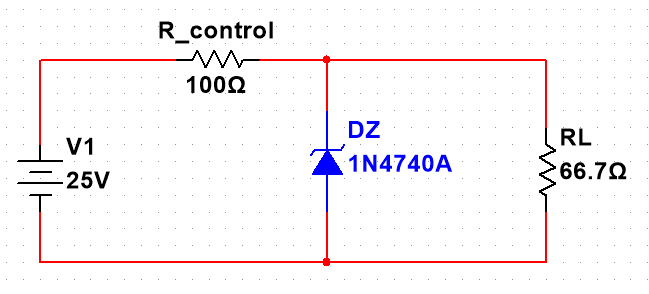
\includegraphics[width=0.45\textwidth]{IMAGENES/SIM_1.png}
\caption{Circuito 1, resistencia mínima.}
\label{fig:SIM_1}
\end {center}
\end{figure}

Resultados obtenidos:

\begin{table}[H]
\centering
\begin{tabularx}{\columnwidth}{|c|X|X|X|}
\hline
\textbf{Componente} & \textbf{$I$ (mA)} & \textbf{$V$ (V)} & \textbf{$P$ (W)}\\ \hline
$RL$ & 149.12 & 9.95  & 1.48\\ \hline
$DZ$ & 1.403 & 9.95  & 0.0139\\ \hline
$R_{\text{control}}$ & 150.53 & 15.053  & 2.26\\ \hline
\end{tabularx}
\caption{Tabla de resultados $RL_{min}$.}
\label{tablaSIM1}
\end{table}

Simulación con resistencia máxima calculada $RL_{max} = 169 \Omega$

\begin{figure}[H]%[!ht]
\begin {center}
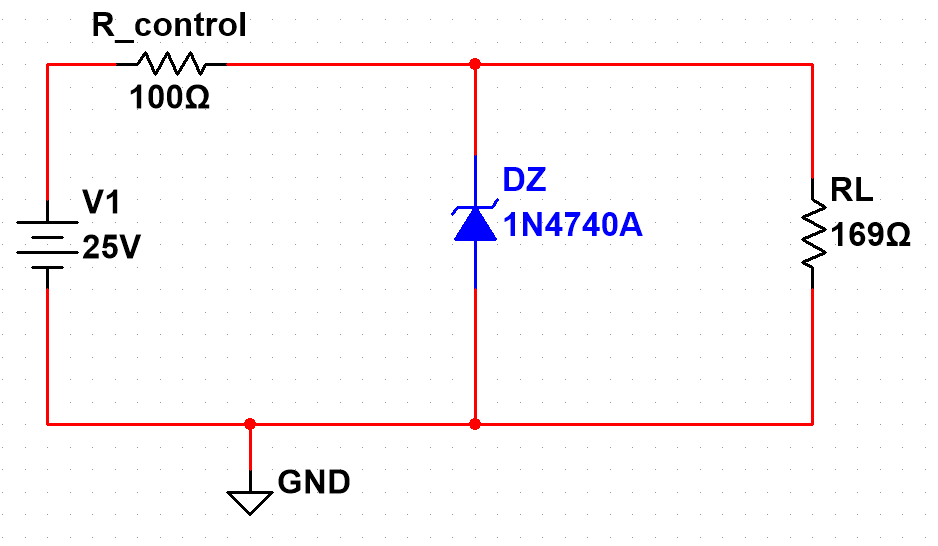
\includegraphics[width=0.45\textwidth]{IMAGENES/SIM_2.png}
\caption{Circuito 1, resistencia máxima.}
\label{fig:SIM_2}
\end {center}
\end{figure}

Resultados obtenidos:

\begin{table}[H]
\centering
\begin{tabularx}{\columnwidth}{|c|X|X|X|}
\hline
\textbf{Componente} & \textbf{$I$ (mA)} & \textbf{$V$ (V)} & \textbf{$P$ (W)}\\ \hline
$RL$ & 59.35 & 10.03  & 0.595\\ \hline
$DZ$ & 90.348 & 10.03  & 0.906\\ \hline
$R_{\text{control}}$ & 149.7 & 14.97  & 2.24\\ \hline
\end{tabularx}
\caption{Tabla de resultados $RL_{max}$.}
\label{tablaSIM2}
\end{table}

Como podemos observar, en los calculos anteriores asumimos un voltaje en el diodo de 10V consstantes. Sin embargo, en la simulación muestra que el voltaje varía entre 9.95V y 10.03V. 
Debido a esto, la corriente en los componentes también se ve afectada, variando ligeramente en lugar de mantenerse fija en 150 mA. Y por último, en el cáñculo teórico para $RL_{min}$
se forzó al zener a operar con su corriente de codo ideal de 0.25 mA, sin embargo, en la simulación, la corriente real que fluye por el diodo es de 1.405 mA, indicando que el  modelo SPICE
del componente requeire un poco más de corriente que la ideal para sotenter la regulación cerca de los 10V.

\subsection{Circuito 2. Valores máximos y mínimos de $V1$}
Simulación con voltaje mínimo calculado $V1_{min} = 12.525 V$

\begin{figure}[H]%[!ht]
\begin {center}
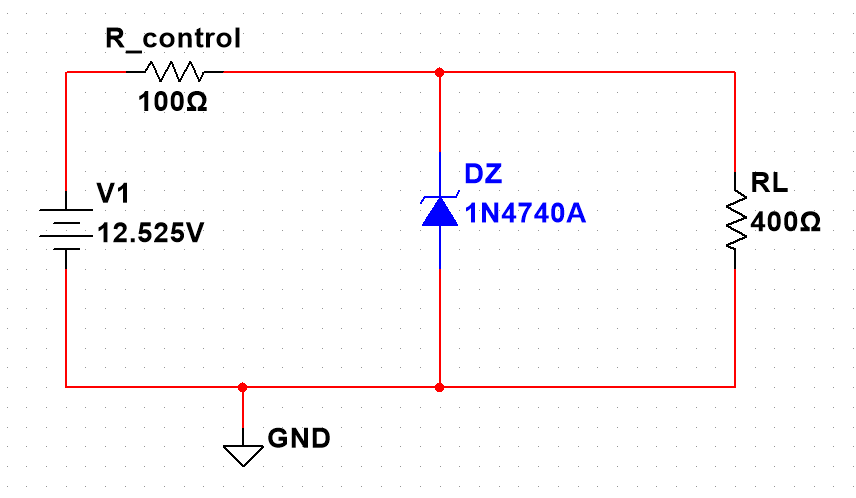
\includegraphics[width=0.45\textwidth]{IMAGENES/SIM_3.png}
\caption{Circuito 2, voltaje mínimo.}
\label{fig:SIM_3}
\end {center}
\end{figure}

Resultados obtenidos:

\begin{table}[H]
\centering
\begin{tabularx}{\columnwidth}{|c|X|X|X|}
\hline
\textbf{Componente} & \textbf{$I$ (mA)} & \textbf{$V$ (V)} & \textbf{$P$ (W)}\\ \hline
$RL$ & 24.813 & 9.925  & 0.246\\ \hline
$DZ$ & 1.185 & 9.925  & 0.011\\ \hline
$R_{\text{control}}$ & 25.998 & 2.6  & 0.067\\ \hline
\end{tabularx}
\caption{Tabla de resultados $V1_{min}$.}
\label{tablaSIM3}
\end{table}

Simulación con voltaje máximo calculado $V1_{max} = 21.6 V$

\begin{figure}[H]%[!ht]
\begin {center}
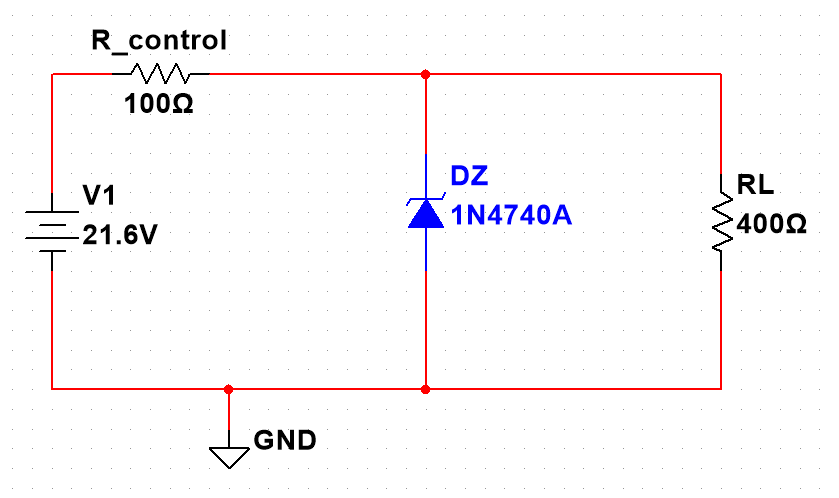
\includegraphics[width=0.45\textwidth]{IMAGENES/SIM_4.png}
\caption{Circuito 2, voltaje máximo.}
\label{fig:SIM_4}
\end {center}
\end{figure}

Resultados obtenidos:

\begin{table}[H]
\centering
\begin{tabularx}{\columnwidth}{|c|X|X|X|}
\hline
\textbf{Componente} & \textbf{$I$ (mA)} & \textbf{$V$ (V)} & \textbf{$P$ (W)}\\ \hline
$RL$ & 25.094 & 10.037  & 0.251\\ \hline
$DZ$ & 90.532 & 10.037  & 0.908\\ \hline
$R_{\text{control}}$ & 115.625 & 11.563  & 1.33\\ \hline
\end{tabularx}
\caption{Tabla de resultados $V1_{max}$.}
\label{tablaSIM4}
\end{table}

Podemos observar en este caso que al aplicar el $V1_{min}$ calculado, el voltaje en la resistencia de carga $RL$ no alcanza los 10 V, quedandose muy cerca en 9.925 V. Como consecuencia, la corriente en la carga varía 
dando un resultado de 24.813 mA, en lugar de los 25 mA que se esperaba. Por otro lado, al probar el $V1_{max}$ el voltaje regulado superó ligeramente el valor nominal, obteniendo un valor de 10.037 V, lo que
resulta en que el diodo zener absorve una corriente de 90.523 mA, lo que es un valor cercano al esperado teorico de 91 mA, validandio el diseño para el caso de estrés máximo.

En conclusión, los cácluculos teóricos son una buena herramienta para aproximar los valores de diseños como las resistencias de protección y rangos de voltaje, pero en la realidad, en las aplicaciones críticas se debe contemplar la
resistencia dinámica del componente para predecir las caídas de voltaje reales y las corrientes que fluirán por el circuito, para así evitar daños en los componentes o un mal funcionamiento del circuito.


\section*{a) Análisis de las regiones directa e inversa}

Analizar las variaciones de las regiones inversas y directas que existen en ambos 
diodos, y describir lo observado a medida que aumenta la temperatura.

En la región inversa de ambos diodos, a simple vista la corriente parece mantenerse como 
una línea recta constante en $0\,A$. Sin embargo, al ampliar la escala dentro de la simulación, 
se nota la presencia de pequeñas corrientes de fuga (la línea no es completamente plana). 

En el caso del 1N4148, a medida que aumenta la temperatura, la corriente inversa 
comienza a incrementarse incluso antes de llegar a los $0\,V$.

Por otro lado, en las regiones directas se puede apreciar cómo en el 1N4001 la corriente 
crece de manera estable. Además, es evidente que, a mayor temperatura, el diodo 
disminuye su barrera de potencial y no necesita tanto voltaje para empezar a conducir 
corriente.

\section*{b) Comparación del comportamiento térmico}

Comparar el comportamiento de ambos diodos y determinar cuál tiene un 
comportamiento más lineal con respecto a la temperatura.

Se puede observar en las gráficas cómo las curvas del 1N4001 se mantienen prácticamente 
paralelas entre sí en todos los casos de temperatura; es decir, mantiene un comportamiento 
lineal constante sin importar los incrementos térmicos. 

Por otro lado, el 1N4148 no se mantiene constante, sino que la pendiente de la curva cambia 
drásticamente entre cada variación de temperatura.

En conclusión, el diodo 1N4001 tiene un comportamiento más lineal y predecible con 
respecto a la temperatura en su región de conducción. Esto se debe a que es un diodo 
rectificador de potencia (diseñado para manejar mayores corrientes y disipar calor de forma 
estable), mientras que el 1N4148 es un diodo de pequeña señal y conmutación rápida, cuya 
unión es más pequeña y, por ende, más sensible a cambios térmicos drásticos.

\section*{d) Rangos de operación y aplicaciones}

\subsection*{Diodo Rectificador 1N4001}

\begin{itemize}
    \item \textbf{Rango de temperatura de operación (según hoja de datos):} $-55\,^{\circ}C$ a $+150\,^{\circ}C$ (temperatura de la unión).
    \item \textbf{Aplicaciones:} Uso general. Está diseñado para rectificar corriente alterna a 
    corriente directa a bajas frecuencias (como en fuentes de alimentación de 50/60 Hz), 
    protección contra polaridad inversa y en circuitos donde se manejan corrientes de 
    hasta $1\,A$ y voltajes de conmutación no muy rápidos.
\end{itemize}

\subsection*{Diodo de Señal 1N4148}

\begin{itemize}
    \item \textbf{Rango de temperatura de operación (según hoja de datos):} $-65\,^{\circ}C$ a $+150\,^{\circ}C$ 
    (en algunos empaques de vidrio soporta hasta $+200\,^{\circ}C$).
    \item \textbf{Aplicaciones:} Conmutación rápida (\textit{fast switching}). Se utiliza en procesamiento de 
    señales de alta frecuencia, circuitos lógicos digitales, multiplicadores de voltaje de 
    pequeña señal y en sistemas donde se requiere que el diodo cambie de estado (de 
    conducir a no conducir) en tiempos muy cortos (nanosegundos).
\end{itemize}

\section{Conclusiones}
\begin{itemize}
    \item \textbf{Flores Cornejo Gustavo Mauricio.}
    \newline En la presente práctica se pone en evidencia el comportamiento de 2 tipos de diodos de silicio, por lo que su comportamiento, como se puede ver en el desarrollo de la 
    práctica, es muy similar. Esta práctica sirve como base para comprender mucha de la parte teórica del diodo, como lo es su variación de parámetros al alterar la temperatura, además de visualizar el comportamiento de un diodo 
    real y comparalo con el comportamiento ideal. Como lo vimos en la sección del osciloscopio podemos observar una diagonal que representa el comportamiento del diodo cuando se encunetra polarizado inversamente, aquí retomamos el concepto 
    de la corriente de fuga que presenta el diodo. Mientras que el diodo ideal presenta una transición abrupta entre conducción y no conducción, el diodo real muestra una curva exponencial en la región directa y pequeñas corrientes en la región inversa. Como se observó en la sección del osciloscopio, la presencia de una línea diagonal en la región de polarización inversa retoma el concepto de la corriente de fuga, demostrando que el dispositivo no se comporta como un interruptor perfecto.

Finalmente, el análisis comparativo permitió entender que, aunque ambos diodos están fabricados en silicio, su diseño y aplicación influyen en su sensibilidad térmica y comportamiento eléctrico.
    
    \item \textbf{Muñoz Reyes Arturo Yabet.}
    \newline En conclusión, esta práctica comprobó de manera efectiva el comportamiento unidireccional y las características eléctricas de los diodos 1N4001 y 1N4148. Mediante mediciones se comprobó su funcionamiento en polarización directa e inversa, confirmando 
    que requieren un voltaje de activación típico de entre 0.6 V y 0.7 V para conducir la corriente. Finalmente, las simulaciones con variaciones de temperatura demostraron la sensibilidad térmica de estos componentes, destacando que el diodo  1N4001 mantiene una 
    mayor estabilidad frente al calor en comparación con el diodo 1N4148. Estos resultados subrayan la importancia de considerar tanto las especificaciones eléctricas como el comportamiento térmico al seleccionar semiconductores para aplicaciones en mecatrónica.

    \item \textbf{Morales Vásquez Miguel Ehecatl.} 
    \newline Tras la realización de esta práctica, se validó experimentalmente que el diodo semiconductor no presenta un comportamiento lineal, ya que requiere superar un voltaje de umbral (entre 0.5 y 0.7V para silicio) para permitir el flujo de corriente. 
    A través del contraste entre los modelos 1N4001 y 1N4148, se comprobó que mientras el primero es óptimo para rectificación de potencia por su capacidad de corriente, el segundo destaca en aplicaciones de alta frecuencia debido a su reducido tiempo de recuperación inversa. 
    Finalmente, el uso del osciloscopio en modo XY y la aplicación de la Ecuación de Shockley permitieron verificar cómo variables externas, especialmente la temperatura, alteran la barrera de potencial y la corriente de fuga, consolidando la comprensión de estos dispositivos en condiciones reales de operación

\end{itemize}



% if have a single appendix:
%\appendix[Proof of the Zonklar Equations]
% or
%\appendix  % for no appendix heading
% do not use \section anymore after \appendix, only \section*
% is possibly needed

% use appendices with more than one appendix
% then use \section to start each appendix
% you must declare a \section before using any
% \subsection or using \label (\appendices by itself
% starts a section numbered zero.)
%


\appendices
\section{Evidencias}





% references section

% can use a bibliography generated by BibTeX as a .bbl file
% BibTeX documentation can be easily obtained at:
% http://mirror.ctan.org/biblio/bibtex/contrib/doc/
% The IEEEtran BibTeX style support page is at:
% http://www.michaelshell.org/tex/ieeetran/bibtex/
%\bibliographystyle{IEEEtran}
% argument is your BibTeX string definitions and bibliography database(s)
%\bibliography{IEEEabrv,../bib/paper}
%
% <OR> manually copy in the resultant .bbl file
% set second argument of \begin to the number of references
% (used to reserve space for the reference number labels box)

%use following command to generate the list of cited references

\printbibliography

\begin{thebibliography}{00}
\bibitem{boylestad}
R. L. Boylestad and L. Nashelsky, \textit{Electronic Devices and Circuit Theory}, 10th ed. Upper Saddle River, NJ, USA: Prentice Hall, 2009.

\bibitem{1N4001}
onsemi, ``1N4001 -- 1.0 A Standard Recovery Rectifier,'' Datasheet, 2023. [Online]. Available: https://www.onsemi.com/pdf/datasheet/1n4001-d.pdf. [Accessed: Feb. 24, 2026].

\bibitem{1N4148}
onsemi, ``1N4148 -- Small Signal Switching Diode,'' Datasheet, 2023. [Online]. Available: https://www.onsemi.com/pdf/datasheet/1n4148-d.pdf. [Accessed: Feb. 24, 2026].
\end{thebibliography}

% that's all folks
\end{document}